\documentclass{article}
\usepackage{url}
\usepackage{amsmath,bm}%
\usepackage{amsfonts}%
\pagestyle{empty}
\setlength{\textwidth}{6.5in}
\setlength{\oddsidemargin}{-.25in}
\setlength{\evensidemargin}{-.25in}
\setlength{\topmargin}{-.5in}
\setlength{\textheight}{9in}

\newcommand{\beaa}{\begin{eqnarray*}}
\newcommand{\eeaa}{\end{eqnarray*}}
\newcommand{\bea}{\begin{eqnarray}}
\newcommand{\eea}{\end{eqnarray}}
\def\E{\mathop{\rm E\,}\nolimits}
\def\Var{\mathop{\rm Var\,}\nolimits}
\def\Cov{\mathop{\rm Cov\,}\nolimits}
\def\Corr{\mathop{\rm Corr\,}\nolimits}
\def\logit{\mathop{\rm logit\,}\nolimits}
\newcommand{\eid}{{\stackrel{\cal{D}}{=}}}
\newcommand{\cip}{{\stackrel{{P}}{\to}}}
\def\bR{\mathbb{R}}     % real line

%%%%%%%%%%
% From http://www.disc-conference.org/disc1998/mirror/llncs.sty
\def\vec#1{\mathchoice{\mbox{\boldmath$\displaystyle\bf#1$}}
{\mbox{\boldmath$\textstyle\bf#1$}}
{\mbox{\boldmath$\scriptstyle\bf#1$}}
{\mbox{\boldmath$\scriptscriptstyle\bf#1$}}}
%%%%%%%%%%

\usepackage{Sweave}
\begin{document}

\begin{center}
{\bf STAT 515}

{\bf Homework \#11 WITH SOLUTIONS}

\end{center}

\begin{enumerate}

  \item Suppose that $Y_1, \ldots, Y_n$ is a simple random sample from
  $N(\theta, 1)$, where we assume that $(\log \theta-\mu)/\sigma$ has a
  $t$~distribution on $r$ degrees of freedom (this is the example we discussed
  briefly in class on April 11). Assume that $\mu$, $\sigma$, and $r$ are known
  (parameters on the prior distribution like this are called {\em
  hyperparameters} in a Bayesian context).
  
    \begin{enumerate}

      \item Describe a Metropolis-Hastings algorithm for sampling from the
      posterior distribution of $\theta\mid \vec Y$, using a normal proposal
      distribution centered at the current value of the Markov chain and with
      variance $\tau^2$.
      \begin{quotation}{\bf Solution:}
      Ignoring multiplicative constants, the likelihood (the joint density for $Y_1, \ldots, Y_n$)
      times the prior for $\theta$ equals
      \[
      \frac1\theta \left[ 1 + \frac1r \left( \frac{\log \theta - \mu}{\sigma} \right)^2 \right] ^{-(r+1)/2} \exp \left\{
      -\frac12 \sum_{i=1}^n (Y_i -\theta)^2 \right\} I\{ \theta>0\}.
      \]
      Let us call this function $\pi(\theta)$ to simplify notation.
      Letting $\theta^*$ denote a proposed next value and $\theta$ the current value of the
      chain, we conclude that a normal proposal distribution as specified leads to a Metropolis-Hastings
      acceptance ratio equal to $\pi(\theta^*)/\pi(\theta)$, since the normal proposal
      density is symmetric (that is, $q(\theta \mid \theta^*)=q(\theta^*\mid \theta)$ if we take
      $q(x \mid y)$ to be a normal density function with mean $y$ evaluated at $x$.
      
      We conclude that the Metropolis-Hastings algorithm consists of first simulating a normal
      random value $\theta^*$ with mean $\theta$ and variance $\tau^2$, then accepting 
      $\theta^*$ (replacing $\theta$ by $\theta^*$) as long as a standard uniform random variable
      is less than $\pi(\theta^*)/\pi(\theta)$.  
      
      However, the algorithm should calculate the ratio on the log scale for the sake of 
      numerical stability.  This means that we accept $\theta^*$ whenever
      \[
      \log U < \log \pi(\theta^*) - \log\pi(\theta).
      \]
      Whenever $\theta^*\le0$, the value of $\pi(\theta^*)$ equals zero, which means that
      we never accept $\theta^*$ in that case.
      \end{quotation}
      
      \item Take $\mu=0$, $\sigma=5$, and $r=4$. For the dataset $Y_1, \ldots,
      Y_{100}$ at
      \url{http://sites.stat.psu.edu/~dhunter/515/hw/hw11prob1b.txt}, implement
      your M-H algorithm starting the chain at $\theta_0=1$ and running for
      50,000 steps. Use $\tau^2=1$.
      \begin{quotation}{\bf Solution:}
      In R:
\begin{Schunk}
\begin{Sinput}
> # First, we create a function to calculate log(pi):
> logpi <- function(x, data, mu=0, sigma=5, r=4) {
+   if (x<0) 
+     return (-Inf)
+   else 
+     return ( -(r+1)/2*log(1 + ((log(x) - mu)/sigma)^2/r) - log(x) - sum((data-x)^2)/2)
+ }
> # Here is a function to return a sample from the posterior:
> samplePosterior <- function(tau=1, n=50000) {
+   y <- scan("http://sites.stat.psu.edu/~dhunter/515/hw/hw11prob1b.txt")
+   theta <- rep(1, 50001) # This will hold the theta values
+   accepts <- 0 # Keep track of the number of acceptances
+   # Here is the main loop:
+   for(i in 1:50000) {
+     thetaStar <- rnorm(1, mean=theta[i], sd=tau)
+     u <- runif(1)
+     if (thetaStar>0 && log(u) < logpi(thetaStar, y) - logpi(theta[i], y)) {
+       accepts <- accepts + 1
+       theta[i+1] <- thetaStar
+     } else {
+       theta[i+1] <- theta[i]
+     }
+   }
+   cat("Acceptance rate: ", accepts / n)
+   return(theta)
+ }
> theta <- samplePosterior(tau=1)
\end{Sinput}
\begin{Soutput}
Acceptance rate:  0.12504
\end{Soutput}
\end{Schunk}
      \end{quotation}
      
      \item Record the acceptance rate of your MH algorithm. Then create a trace
      plot in which you plot the values of $\theta_i$ against $i$. Comment on
      it: Does it appear that your Markov chain is effectively ``mixing''?
      \begin{quotation}{\bf Solution:}
      The acceptance rate was reported above; it is the proportion of
      proposals that were accepted.
      Here is the trace plot:
\begin{Schunk}
\begin{Sinput}
> plot(theta, type="l")
\end{Sinput}
\end{Schunk}
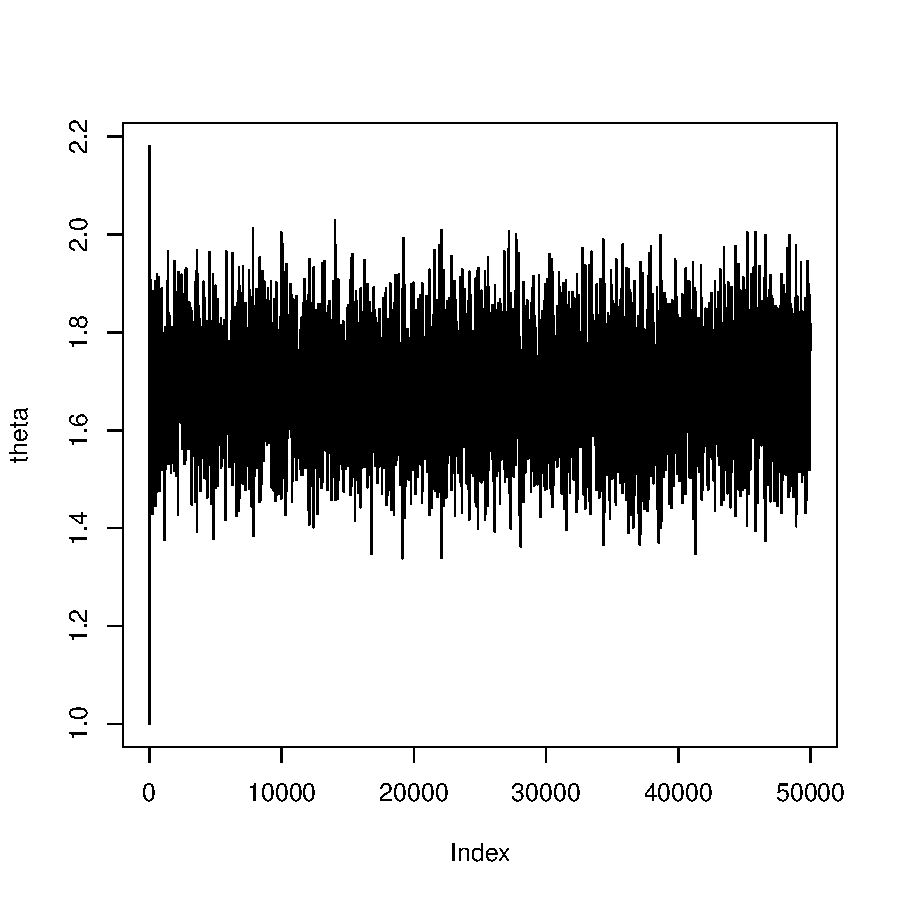
\includegraphics{sol11-002}
      
      This trace plot looks great.  There is no reason to think that this chain is failing to mix well based
      on the plot.
      \end{quotation}
      
      \item Create a histogram of the $\theta_i$ values. Also, report a point
      estimate (the posterior mean) along with a 95\% credible interval for
      $\theta$ based on your posterior sample. (For the latter, just use the
      0.025 and 0.975 sample quantiles of your sample.)
      \begin{quotation}{\bf Solution:}
      Here is a histogram (with a density estimate superimposed):
\begin{Schunk}
\begin{Sinput}
> hist(theta, freq=FALSE)
> lines(density(theta), col=2)
\end{Sinput}
\end{Schunk}
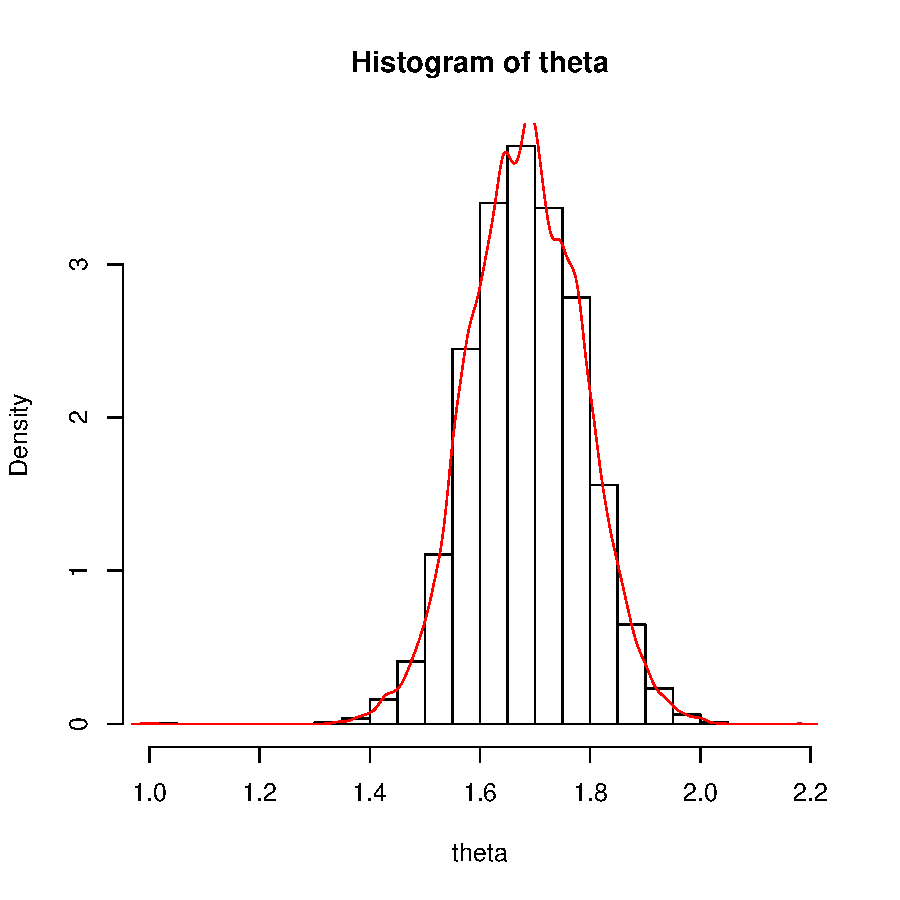
\includegraphics{sol11-003}
      The posterior mean and credible interval consisting of the 0.025 and 0.975
      quantiles are as follows:
\begin{Schunk}
\begin{Sinput}
> mean(theta)
\end{Sinput}
\begin{Soutput}
[1] 1.683853
\end{Soutput}
\begin{Sinput}
> quantile(theta, c(.025, .975))
\end{Sinput}
\begin{Soutput}
    2.5%    97.5% 
1.491092 1.877253 
\end{Soutput}
\end{Schunk}
      This credible interval reflects the uncertainty about the value of $\theta$ 
      intrinsic to the problem.  It does not reflect the uncertainty about the 
      posterior distribution of $\theta$ due to the fact that we're using MCMC to 
      sample from that distribution.  
      \end{quotation}
      
      \item To create a 95\% confidence interval for the true posterior mean, a
      naive idea would be to try
      \[
      \hat\mu \pm \frac{1.96}{\sqrt{n}}*\sqrt{\frac1{n-1}\sum_{i=1}^{50{,}000} (\theta_i - \hat\mu)^2 },
      \]
      where $\hat\mu$ is your point estimate from part (d). Explain why this
      interval has a totally different interpretation than your interval from
      part (d). (Hint: Only one of these intervals tries to capture the MCMC
      error.) Also, explain why this idea is likely to produce an interval that
      is narrower than it should be---and hence, it is not a very good idea from
      a statistical point of view.
      \begin{quotation}{\bf Solution:}
      This interval only reflects uncertainty about the true posterior mean based on 
      {\em this particular sample}.  In other words, the posterior mean is a fixed but unknown
      constant, and we are using a random procedure to try to estimate it, and the confidence
      interval reflects our uncertainty about that fixed value due to the randomness of the procedure.
      It does {\em not} reflect the uncertainty about $\theta$ due to the fact that the $Y_i$
      were randomly chosen to begin with.   (The credible interval in part (d) does that.)
      
      The reason that the confidence interval is too narrow is that the variance of the sample
      mean will include some positive covariances, so it will be larger than the variance
      based on an i.i.d.~sample from the posterior would be.  Yet the naive formula uses
      the i.i.d.~version.
      \end{quotation}
      
      \item Replicate part (c) using a value of $\tau^2$ that appears ``too
      small''. Then do the same thing for a value of $\tau^2$ that appears ``too
      big''. In each case, try to explain why the chain does not appear to be as
      effective as in part (c).
      \begin{quotation}{\bf Solution:}
      Let us try $\tau^2=10^{-6}$ and look at a trace plot:
\begin{Schunk}
\begin{Sinput}
> theta2 <- samplePosterior(tau=1/1000)
\end{Sinput}
\begin{Soutput}
Acceptance rate:  0.99118
\end{Soutput}
\begin{Sinput}
> plot(theta2, type="l")
\end{Sinput}
\end{Schunk}
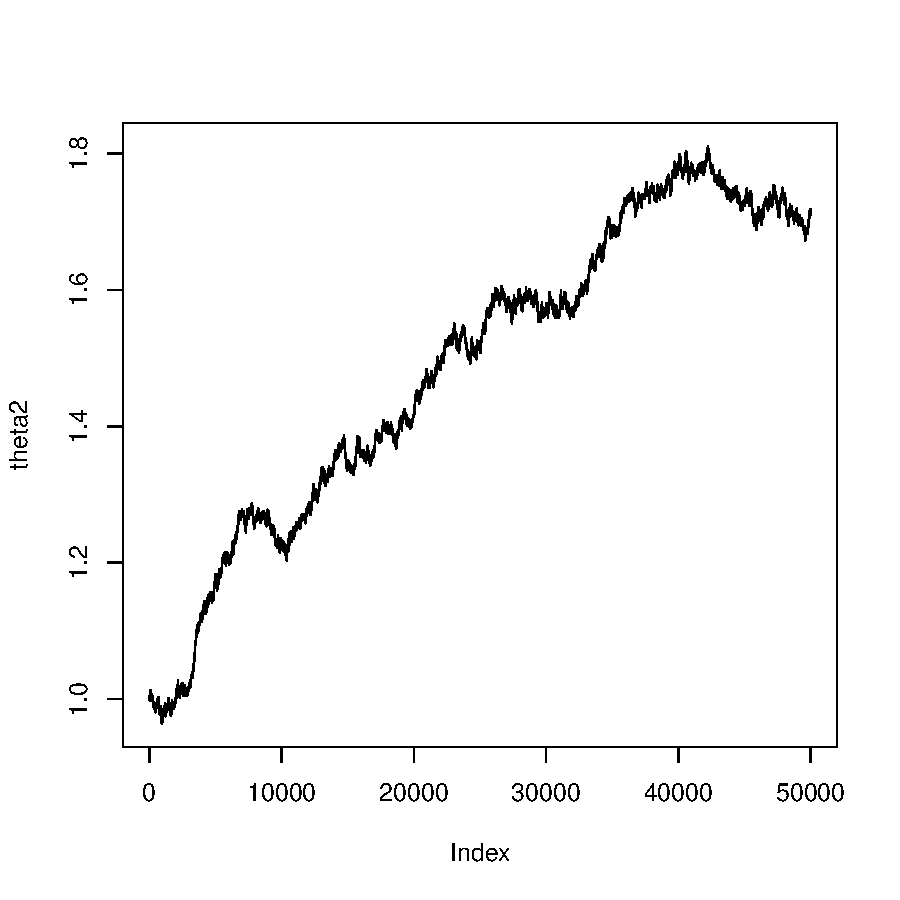
\includegraphics{sol11-005}
      
      Nearly every proposal is accepted, but the traceplot reveals that mixing is very slow.  
      This is because each proposed $\theta^*$ is very close to the current $\theta$.
      
      Next, consider $\tau^2=10^6$:
\begin{Schunk}
\begin{Sinput}
> theta3 <- samplePosterior(tau=1000)
\end{Sinput}
\begin{Soutput}
Acceptance rate:  2e-04
\end{Soutput}
\begin{Sinput}
> plot(theta3, type="l")
\end{Sinput}
\end{Schunk}
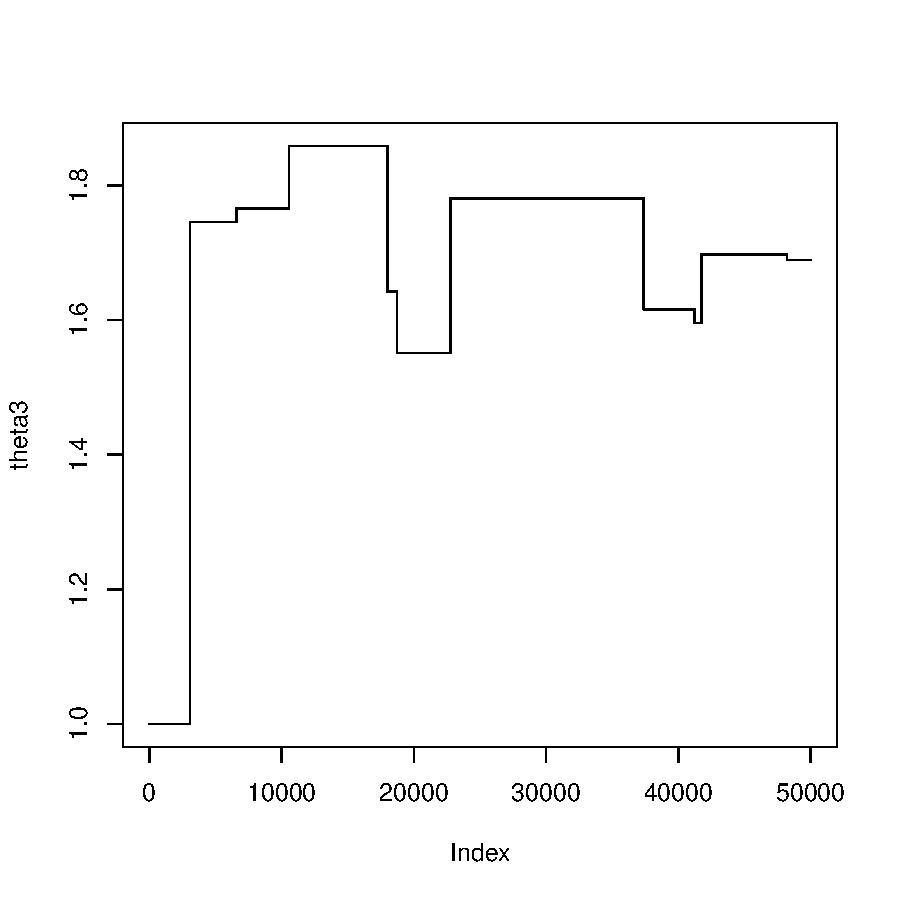
\includegraphics{sol11-006}
      
      In this case, the mixing is very slow because almost none of the proposals are accepted.
      The reason for this is that they are very far away from $\theta$, and the acceptance probability
      is therefore quite low most of the time.
      \end{quotation}

    \end{enumerate}

  \item The goal of this problem is to analyze a dataset in which the
  observations are assumed to come from a piecewise-homogeneous Poisson process
  in which the Poisson rate starts at one value and then changes at some unknown
  time to a different value.

  The data are at 
  \url{http://sites.stat.psu.edu/~dhunter/515/hw/hw11prob2.txt},
  where the events have been binned into 50 time periods of equal length. A
  model, adapted by Murali Haran from Chapter 5 of "Bayes and Empirical Bayes
  Methods for Data Analysis" by Carlin and Louis (2000), for the binned counts
  $Y_1, \ldots, Y_{50}$ is as follows:
  \begin{eqnarray*}
  Y_i \mid k, \theta, \lambda \sim \begin{cases}
  \mbox{Poisson}(\theta) & \mbox{for $i=1, \ldots, k$;} \\
  \mbox{Poisson}(\lambda) & \mbox{for $i=k+1, \ldots, 50$.} \\
  \end{cases}
  \end{eqnarray*}
  The prior distributions on the $k$, $\theta$, and $\lambda$ parameters, along
  with two hyperparameters $b_1$ and $b_2$, are as follows:
  \begin{eqnarray*}
  \theta\mid b_1 &\sim& \mbox{Gamma}(0.5, b_1) \\
  \lambda\mid b_2 &\sim& \mbox{Gamma}(0.5, b_2) \\
  k &\sim& \mbox{Unif}\{1, \ldots, 50\} \\
  b_1 &\sim& \mbox{Inverse Gamma}(0,1) \\
  b_2 &\sim& \mbox{Inverse Gamma}(0,1),
  \end{eqnarray*}
  where $b_1$ and $b_2$ are independent and $k$, $\theta$, and $\lambda$ are
  conditionally independent given $b_1$ and $b_2$. The density functions of the
  Gamma$(\alpha, \beta)$ and Inverse Gamma$(\alpha, \beta)$ distributions are,
  respectively,
  \[
  f(x) = \frac{1}{\Gamma(\alpha)\beta^\alpha} x^{\alpha-1} e^{-x/\beta}
  \quad\mbox{and}\quad
  f(x) = \frac{1}{\Gamma(\alpha)\beta^\alpha} x^{-\alpha-1} e^{-1/(x\beta)}.
  \]
  Please take note:  The stated priors for $b_1$ and $b_2$ are not proper probability
  distributions:  Integrating $\exp\{-1/b)/b$ from 0 to $\infty$ does not converge to a finite
  value.  However, if you simply use the improper prior density $\exp\{-1/b)/b$, you will obtain
  proper full conditional distributions for all of the parameters.
  
  Specific instructions are as follows:

    \begin{enumerate}
    
    \item Derive the full conditional densities or mass functions (up to a
    constant) for each of the five parameters conditional on the other four and
    the data. For $\theta$, $\lambda$, $b_1$, and $b_2$, describe these full
    conditionals as coming from some named parametric family, and give the
    parameters.
    \begin{quotation}{\bf Solution:}
    The joint density of the data and the parameters (ignoring multiplicative constants
    and after some rearranging) is
    \[
    e^{-\theta k}\theta^{S_k}
    e^{-\lambda(n-k)}\lambda^{S_n-S_k}
    \frac{1}{(b_1b_2)^{3/2}} \frac{1}{\sqrt{\theta\lambda}} 
    e^{-1/b_1} e^{-\theta/b_1}
    e^{-1/b_2} e^{-\lambda/b_2},
    \]
    where $S_k=\sum_{i=1}^k Y_i$ for $1\le k \le n$,
    and this may be taken as the full conditional density, up to a constant, for each of the
    five parameters.
    The dependence of this density on $k$ is somewhat complicated; however, each of the
    other four parameters has a recognizable full conditional distribution.  Isolating each
    of them in turn from the product above gives
    \begin{eqnarray*}
    \mbox{For $\theta$:  } & \theta^{S_k - 1/2}
    e^{-\theta(k+1/b_1)}& 
    \mbox{thus, $\theta\sim \mbox{Gamma}\left[ \frac12+S_k, b_1/(1+b_1k) \right]$.} \\
    \mbox{For $\lambda$:  } & \lambda^{S_n-S_k - 1/2}
    e^{-\lambda(n-k+1/b_2)}& 
    \mbox{thus, $\theta\sim \mbox{Gamma}\left[ \frac12+S_n-S_k, 
    b_2/(1+b_2(n-k)) \right]$.} \\
    \mbox{For $b_1$:  } & b_1^{-3/2} e^{-(\theta+1)/b_1} & \mbox{thus, $b_1\sim
    \mbox{Inverse Gamma}\left[  \frac12, 1/(1+\theta) \right] $.} \\
    \mbox{For $b_2$:  } & b_2^{-3/2} e^{-(\lambda+1)/b_2} & \mbox{thus, $b_2\sim
    \mbox{Inverse Gamma}\left[  \frac12, 1/(1+\lambda) \right] $.} \\
    \end{eqnarray*}
    \end{quotation}
    
    \item Implement a one-variable-at-a-time Metropolis-Hastings algorithm to
    sample from the posterior distribution. For $\theta$, $\lambda$, $b_1$, and
    $b_2$, use Gibbs sampling from the full conditionals; for $k$, use a
    Metropolis-Hastings update where the proposal distribution is uniform on
    $\{2, \ldots, 49\}$. Run at least one million iterations of the algorithm.
    \begin{quotation}{\bf Solution:}
    The M-H algorithm is straightforward using the full conditionals in part (a), except 
    the update for $k$, for which the logarithm of the acceptance probability equals
    \[
    (k-k^*)(\theta-\lambda) + (S_{k^*}-S_k)(\log \theta - \log\lambda)
    \]
    In calculating the ratio above, we use the fact that the uniform proposal
    distribution is symmetric, so the ratio is simply $\pi(k^*)/\pi(k)$.
    Here is the code:
\begin{Schunk}
\begin{Sinput}
> m <- 1e6
> # Set up parameter vectors
> Theta <- Lambda <- k <- b1 <- b2 <- rep(1, 1 + m)
> # Read data (only need second column)
> Y <- read.table("http://sites.stat.psu.edu/~dhunter/515/hw/hw11prob2.txt", head=T)[,2]
> cy <- cumsum(Y) # We only need the cumulative sums in the algorithm
> for (i in 1:m) {
+   # First, the 4 Gibbs sampling steps:
+   Theta[i+1] <- rgamma(1, .5+cy[k[i]], scale=b1[i]/(1+k[i]*b1[i]))
+   Lambda[i+1] <- rgamma(1, .5+cy[50]-cy[k[i]], scale=b2[i]/(1+(50-k[i])*b2[i]))
+   b1[i+1] <- 1/rgamma(1, 1/2, rate=1+Theta[i+1])
+   b2[i+1] <- 1/rgamma(1, 1/2, rate=1+Lambda[i+1])
+   # Now the update of k:
+   kstar <- 1+sample(48,1) # Choose uniformly from 2, ..., 49
+   logratio <- (k[i]-kstar)*(Theta[i+1]-Lambda[i+1]) + 
+                    (cy[kstar]-cy[k[i]]) * (log(Theta[i+1]) - log(Lambda[i+1]))
+   if (log(runif(1)) < logratio) {
+     k[i+1] <- kstar
+   } else {
+     k[i+1] <- k[i]
+   }
+ }
\end{Sinput}
\end{Schunk}
    \end{quotation}
    
    \item Give a 95\% credible interval for $k$ (use the 0.025 and 0.975
    quantiles of the posterior distribution of $k$). Then, produce a plot of the
    data (Time vs.~Count) and overlay the mean of the Poisson process on the
    same plot, where this mean is determined by the posterior means of $k$,
    $\theta$, and $\lambda$.
    \begin{quotation}{\bf Solution:}
    Here is the credible interval:
\begin{Schunk}
\begin{Sinput}
> quantile(k, c(.025, .975))
\end{Sinput}
\begin{Soutput}
 2.5% 97.5% 
   30    37 
\end{Soutput}
\end{Schunk}
    In fact, I generated these data using a true value of $k=35$ (and 
    $\theta=16$ and $\lambda=22$), so this procedure 
    based on a sample of only size 50 seems to have worked pretty well.
    Below is a plot of the data with the appropriate means overlaid.
    You may find the text-plotting function useful in the future.
\begin{Schunk}
\begin{Sinput}
> plot(Y, ylab="Count", xlab="")
> abline(v=mean(k), lty=2)
> lines(c(0, mean(k)), rep(mean(Theta), 2), lty=2, lwd=2, col=2)
> lines(c(mean(k), 51), rep(mean(Lambda), 2), lty=2, lwd=2, col=2)
> # Add values of posterior means to plot:
> text(mean(k)+1, min(Y), 
+      as.expression(bquote(bar(k) == .( round(mean(k),2)  ))), 
+      pos=4, cex=1.5)
> text(mean(k)+1, mean(Theta), 
+      as.expression(bquote(bar(theta) == .( round(mean(Theta),2)  ))), 
+      pos=4, cex=1.5)
> text(mean(k)-1, mean(Lambda), 
+      as.expression(bquote(bar(lambda) == .( round(mean(Lambda),2)  ))), 
+      pos=2, cex=1.5)
\end{Sinput}
\end{Schunk}
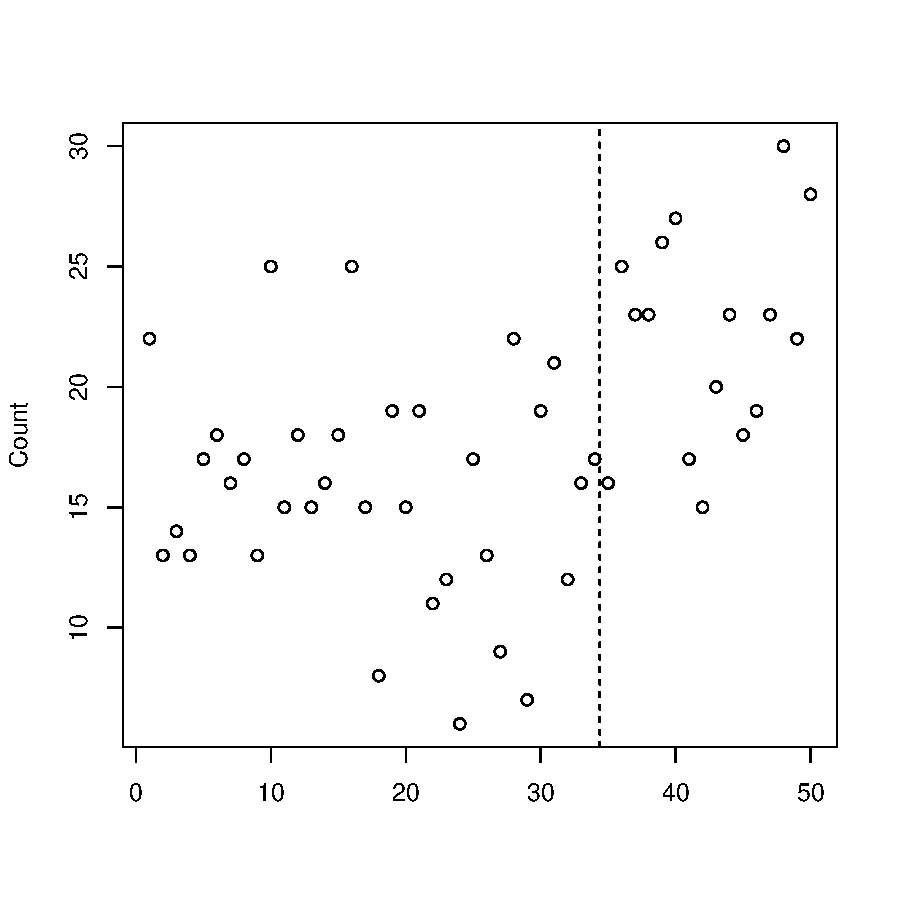
\includegraphics{sol11-009}
    \end{quotation}

    \end{enumerate}

  If you are interested in seeing an application of the model in this problem to
  a real dataset, or if you simply get stuck on this problem, you might find the
  writeup by Murali Haran at 
  \url{http://sites.stat.psu.edu/~mharan/MCMCtut/MCMC.html} to be helpful.

\end{enumerate}

\end{document}

